\documentclass[conference]{IEEEtran}
\IEEEoverridecommandlockouts
% The preceding line is only needed to identify funding in the first footnote. If that is unneeded, please comment it out.
\usepackage{cite}
\usepackage{amsmath,amssymb,amsfonts}
\usepackage{algorithmic}
\usepackage{graphicx}
\usepackage{textcomp}
\usepackage{xcolor}
\usepackage{subcaption}

\usepackage[hyphenbreaks]{breakurl}
\usepackage[hyphens]{url}

% spanish symbols for narrative
\usepackage[utf8]{inputenc} 
% language
\usepackage[spanish]{babel} 

%changing from roman number to integers
\renewcommand{\thesection}{\arabic{section}}
\renewcommand{\thesubsection}{\arabic{section}.\arabic{subsection}} 
\renewcommand{\thetable}{\arabic{table}}
%\renewcommand\topfraction{.9}
%\renewcommand\textfraction{0.35}
%\renewcommand\floatpagefraction{0.8}

\usepackage{pgfplots}
\usepackage{pgfplotstable}
    \pgfplotsset{
        % use this `compat' level or higher to position the bars in one group
        % next to each other
        compat=1.7,
    }
    % load the data table ...
    \pgfplotstableread[col sep=comma]{misc/dtFemaleAgeDistribution.csv}{\femaleAgeDistribution}
        % and store the number of columns in `\NoOfCols'
        % (minus 1 because counting in `\foreach' starts with zero
        \pgfplotstablegetcolsof{\femaleAgeDistribution}
        \pgfmathtruncatemacro{\NoOfCols}{\pgfplotsretval-1}
    % load the data table ...
    \pgfplotstableread[col sep=comma]{misc/dtMaleAgeDistribution.csv}{\maleAgeDistribution}
        % and store the number of columns in `\NoOfCols'
        % (minus 1 because counting in `\foreach' starts with zero
        \pgfplotstablegetcolsof{\femaleAgeDistribution}
        \pgfmathtruncatemacro{\NoOfCols}{\pgfplotsretval-1}

%packages used for models diagrams
\usepackage{tikz}
\usetikzlibrary{babel}
\usetikzlibrary{shapes.geometric}
\usetikzlibrary{arrows.meta,arrows}
\usepackage[T1]{fontenc}
\usepackage{textcomp}
\usepackage[left=2cm,right=2cm]{geometry}
\usepackage{graphicx}
\usepackage{amsmath}
\usepackage{pifont}
\usepackage{adjustbox}

\def\BibTeX{{\rm B\kern-.05em{\sc i\kern-.025em b}\kern-.08em
    T\kern-.1667em\lower.7ex\hbox{E}\kern-.125emX}}
\begin{document}
\title{Automatización de evaluación de madurez ósea a través de técnicas de aprendizaje profundo\\
}

%\author{\IEEEauthorblockN{Autores}
%\IEEEauthorblockA{
%\textit{Grupo de Investigación de Aprendizaje Profundo} \\
%\textit{Departamento Ingeniería en Sistemas de Información}\\
%\textit{Universidad Tecnológica Nacional}\\
%\textit{Facultad Regional Rosario}\\
%mail@frro.utn.edu.ar} %should be hyperlink
%}

\maketitle

%\renewcommand{\abstractname}{Abstract} %Ajustes por traducción a español
%\begin{abstract}
%
%This document is a model and instructions for \LaTeX.
%This and the IEEEtran.cls file define the components of your paper [title, text, heads, etc.]. *CRITICAL: Do Not Use Symbols, Special Characters, Footnotes, or Math in Paper Title or Abstract.
%\end{abstract}

%\renewcommand{\IEEEkeywordsname}{Palabras Clave} %Ajustes por traducción a español
%\begin{IEEEkeywords}
%aprendizaje profundo, red neuronal convolucional, rsna, procesamiento de imagenes
%\end{IEEEkeywords}

\section*{Abstract}

\textit
{
La evaluación de la edad ósea esquelética es una práctica clínica comúnmente utilizada para investigar la madurez del sistema esquelético de un niño. Esta práctica puede ayudar a los médicos a diagnosticar afecciones que retrasan o aceleran el crecimiento y desarrollo físico. Recientemente, el advenimiento y la proliferación de redes neuronales convolucionales (RNC) ha mostrado ser prometedor en una variedad de aplicaciones de imágenes médicas. En este documento proponemos y probamos varios enfoques de aprendizaje profundo para evaluar la madurez ósea de forma automática comparando dos enfoques: por un lado, una RNC general que estima madurez ósea sobre radiografías de género masculino y femenino; por el otro, dos RNC especializadas cada una en su género respectivo. Los resultados mostraron que la utilización de un modelo general ofrece resultados más precisos para la estimación de madurez ósea; sin embargo, los modelos especializados ofrecer resultados similares. Esta es una de las primeras evaluaciones automatizadas de la edad ósea esquelética probada en un conjunto de datos públicos donde se evalúa la utilización de una RNC general y dos RNC específicas para el género de la persona, para los cuales el código fuente está disponible, representando así una base exhaustiva para futuras investigaciones en el campo.
}

\section{Introducción}

Durante el desarrollo del organismo de una persona, los huesos del esqueleto cambian de tamaño y forma, los cuales responden a una determinada edad ósea. Diferencia entre la edad ósea estimada de un niño y su edad cronológica podría indicar trastornos del crecimiento y anomalías endocrinas \cite{AproachToSkeletalMaturation}. Los médicos utilizan la evaluación de la edad ósea para estimar la madurez del sistema esquelético de un niño. Los métodos de evaluación de la edad ósea generalmente comienzan con tomar una sola imagen de rayos X de la mano izquierda desde la muñeca hasta las puntas de los dedos, ver Figura~\ref{fig:mano}. Los huesos en la imagen de rayos X se comparan con radiografías en un atlas estandarizado de desarrollo óseo. Tal atlas de edad ósea se basa en un gran número de radiografías recogidas de niños del mismo sexo y edad.

\begin{figure}[ht!]
  \centering
  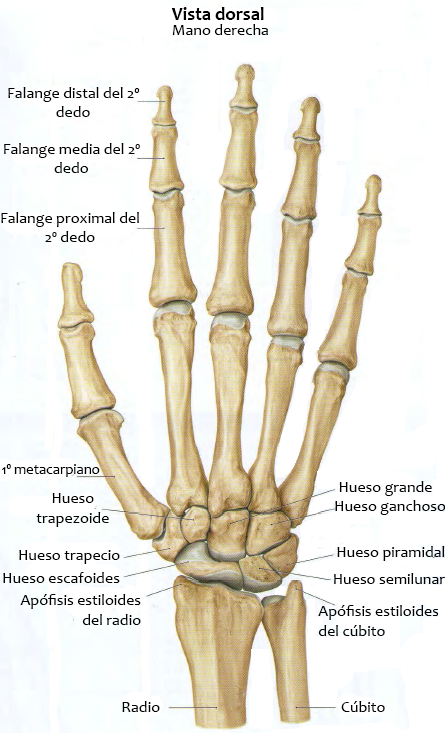
\includegraphics[scale=0.7]{misc/imgHuesosMano.png}
  \caption{Huesos de una mano y muñeca humana adaptada de \cite{AtlasMedicina}}
  \label{fig:mano}
\end{figure}

En las últimas décadas, el procedimiento de evaluación de la edad ósea se realizó de forma manual utilizando los métodos de Greulich y Pyle (GP) \cite{GP} o de Tanner-Whitehouse (TW) \cite{TW3}. El procedimiento GP determina la edad ósea al comparar la radiografía del paciente con un atlas de edades representativas. La técnica TW se basa en un sistema de puntuación que examina 20 huesos específicos. En ambos casos, el procedimiento de evaluación ósea requiere un tiempo considerable; a su vez, la precisión en la estimación depende de la experiencia del radiólogo y tiende a ser subjetiva. 

Desde 1992, preocupaciones sobre la variabilidad interobservador en la estimación manual de la edad ósea \cite{GP_variability} han llevado al establecimiento de varios métodos automáticos computarizados para la estimación de la misma. Los recientes avances en el aprendizaje profundo y sus aplicaciones a la visión por computadora permitieron a muchos investigadores mejorar drásticamente los resultados obtenidos con los sistemas de procesamiento de imágenes particularmente relacionados con el análisis de imágenes médicas \cite{DeepLearningInBiology}. A diferencia de las técnicas tradicionales de aprendizaje automático, las técnicas de aprendizaje profundo permiten que un algoritmo se programe a sí mismo aprendiendo de las imágenes dadas a un gran conjunto de datos de ejemplos etiquetados, eliminando así la necesidad de especificar reglas \cite{DeepLearning}. Los enfoques basados en aprendizaje profundo están ganando más atención porque en varios casos se demostró que logran e incluso superan el rendimiento a nivel humano, lo que hace que el procesamiento de imágenes de extremo a extremo sea automatizado y suficientemente rápido. En el campo de las imágenes médicas, las redes neuronales convolucionales (RNC) se han utilizado con éxito para el cribado de retinopatía diabética \cite{DeepLearningInDiabetics}, diagnóstico de enfermedades cardíacas \cite{DeepLearningInHeartDiseases}, detección de cáncer de pulmón \cite{DeepLearningLungCancer} y otras aplicaciones \cite{DeepLearningInBiology}. En el caso de la evaluación de la edad ósea, el mismo es un procedimiento que realizado manualmente requiere alrededor de 30 minutos de tiempo del médico por cada paciente. Cuando se realiza el mismo procedimiento utilizando un software basado en los métodos clásicos de visión por computadora, toma de 1 a 5 minutos, pero aún requiere una considerable supervisión y experiencia médica. Los métodos basados en aprendizaje profundo permiten evitar la ingeniería de características al aprender automáticamente la jerarquía de características discriminatorias directamente de un conjunto de ejemplos etiquetados. Usando un enfoque de aprendizaje profundo, el procesamiento de una imagen generalmente toma menos de 1 segundo, mientras que la precisión de estos métodos en muchos casos excede la de los métodos convencionales. Soluciones de redes neuronales profundas para la evaluación de la edad ósea de radiografías de mano han sido sugeridas \cite{DeepLearningAssesingSkeletalMaturity1,DeepLearningAssesingSkeletalMaturity2,DeepLearningAssesingSkeletalMaturity3}. Sin embargo, ninguno de estos ha evaluado en profundidad la conveniencia de separar el conjunto de datos de acuerdo al género de la radiografía y generar una RNC por cada género para investigar la precisión resultante de los mismos. 

En este trabajo se investiga si una RNC especializada en un determinado género podría ser más precisa en estimar la edad de una persona de acuerdo a la radiografía de su mano en lugar de una que utilice radiografías de ambos géneros. Nuestra contribución consiste en explorar el comportamiento de una RNC de acuerdo al conjunto de datos que es ingresado en la misma. Validamos la precisión de estas redes neuronales utilizando los datos de el desafío pediátrico de edad ósea 2017 organizado por la Sociedad Radiológica de América del Norte (RSNA) \cite{RSNAChallenge}. Este conjunto de datos ahora está disponible de manera gratuita y puede ser accedido en \cite{RSNADataSet}.

\section{Metodología y Objetivos}

Se realizó la comparación de dos alternativas: por un lado, un modelo general entrenado con radiografías de ambos géneros; y por otro, dos modelos entrenados cada uno con radiografías de un solo género, resultando así la obtención de un modelo específico para cada sexo: uno especializado en radiografías femeninas y otro en radiografías masculinas. El objetivo planteado es analizar cuál de las dos alternativas obtiene mayor precisión: dos modelos especializados en un género cada uno, donde se reduce el conjunto de datos a la mitad o un solo modelo general entrenado con radiografías de ambos géneros. La precisión de los modelos será definida en base al cálculo del MAE (Mean Absolute Error, Error Medio Absoluto) el cual es calculado como $\dfrac{1}{n}\sum\limits_{t=1}^{n}|e_t|$, siendo $|e_t|$ el valor absoluto de la diferencia entre cada estimación y la edad en meses etiquetada en cada observación y $n$ la cantidad de observaciones tomadas.

\subsection{Conjunto de datos}

El conjunto de datos utilizado ha sido extraído del desafío pediátrico de edad ósea 2017 organizado por la Sociedad Radiológica de América del Norte (RSNA) \cite{RSNAChallenge}. El mismo se encuentra conformado por más de 12 mil radiografías pediátricas de muñeca y mano etiquetadas por su género respectivo. Además, el conjunto posee una etiqueta de edad en meses estimada del paciente por un radiólogo. Al realizar la conversión de meses a años, las radiografías del conjunto de datos varían entre 0 y 19 años.
Radiografías de pacientes con una maduración esquelética estimada menor a dos años han sido excluidas del experimento por dos razones. En primer lugar, el conjunto de datos correspondiente a esos rangos de maduración es muy pequeño (38 casos para femenino y 53 casos para masculino). En segundo lugar, la estimación de maduración esquelética es mayormente utilizada para casos de pubertad retrasada, pubertad precoz o baja estatura. Estos estudios raramente son realizados en tales rangos etarios, donde además, se evita la exposición a rayos X.
El número total de observaciones originalmente obtenidas fue de 6,833 para hombres y 5,778 para mujeres. Luego de excluir aquellas de edades entre 0 y 2, ha resultado en 6,780 para hombres y 5,740 para mujeres como se muestra en la Figura~\ref{fig:distribucionEdades}.

% used PGFPlots v1.14
\begin{figure}%[htp]

  \centering
  %\mbox{
  
  \begin{subfigure}{.5\textwidth}
  \centering
	\begin{tikzpicture}
    	\begin{axis}[
        	% adjust the `width' a bit by keeping the default `height'
        	width=1.05*\axisdefaultwidth,
        	height=\axisdefaultheight,
        	% set appropriate `ymax' value so the `nodes near coords' fit to the plot
        	% (adjusting the `ymin' value is just to make it look a little bit better)
        	ymin=0,
        	ymax=2000,
        	% there should be no gap between the bars in one group
        	ybar=0pt,
        	% use data from the table for the xticklabels
        	xtick=data,
        	xlabel=Años,
        	ylabel=Número de radiografías,
        	xticklabels from table={\femaleAgeDistribution}{Anio},
        	% adjust the size of the bars so they don't overlap
        	% (you can play with the numerator to change the gap between the groups)
        	bar width=0.6/\NoOfCols,
        	% enlarge the x limits so all of the bars are shown
        	% (play with the value to adjust the gap on the sides of the plot)
        	enlarge x limits={abs=0.6},
        	% and position the legend outside of the plot to not overlap with the data
        	%legend pos=outer north east,
        	% add `nodes near coords'
        	nodes near coords={
            	% because internally PGFPlots works with floating point numbers, we
            	% change them to fixed point numbers
            	\pgfkeys{
                	/pgf/fpu=true,
                	/pgf/fpu/output format=fixed,
            	}
            	% truncate value count to integer
            	\pgfmathparse{\pgfplotspointmeta}
            	\pgfmathprintnumber{\pgfmathresult}\,
        	},
        	% set the style of the `nodes near coords'
        	nodes near coords style={
            	font=\tiny,
            	rotate=90,
            	anchor=west,
        	},
        	% as basis for the `nodes near coords' use the raw y values
        	point meta=rawy,
        	ymin=1,
    	]
        	% add the data rows for each column 
        	\foreach \i in {1,...,\NoOfCols} {
            	\addplot table [
                	x expr=\coordindex,
                	y index=\i,
                	col sep=comma,
            	] {\femaleAgeDistribution};
                	% to automatically add the legend entries first extract the
                	% column name and store it in `\colname'
                    	\pgfplotstablegetcolumnnamebyindex{\i}\of{\femaleAgeDistribution}\to{\colname}
                	% now you can add the legend entry
                	% (because we are in a loop we have to use the "expanded" version)
                	%\addlegendentryexpanded{\colname};
        	}
    	\end{axis}
    	
	\end{tikzpicture}
  \caption{Femenino}
  \end{subfigure}
  \begin{subfigure}{.5\textwidth}
  \centering
	\begin{tikzpicture}
    	\begin{axis}[
        	% adjust the `width' a bit by keeping the default `height'
        	width=1.05*\axisdefaultwidth,
        	height=\axisdefaultheight,
        	% set appropriate `ymax' value so the `nodes near coords' fit to the plot
        	% (adjusting the `ymin' value is just to make it look a little bit better)
        	ymin=0,
        	ymax=2000,
        	% there should be no gap between the bars in one group
        	ybar=0pt,
        	% use data from the table for the xticklabels
        	xtick=data,
        	xlabel=Años,
        	ylabel=Número de radiografías,
        	xticklabels from table={\maleAgeDistribution}{Anio},
        	% adjust the size of the bars so they don't overlap
        	% (you can play with the numerator to change the gap between the groups)
        	bar width=0.6/\NoOfCols,
        	% enlarge the x limits so all of the bars are shown
        	% (play with the value to adjust the gap on the sides of the plot)
        	enlarge x limits={abs=0.6},
        	% and position the legend outside of the plot to not overlap with the data
        	%legend pos=outer north east,
        	% add `nodes near coords'
        	nodes near coords={
            	% because internally PGFPlots works with floating point numbers, we
            	% change them to fixed point numbers
            	\pgfkeys{
                	/pgf/fpu=true,
                	/pgf/fpu/output format=fixed,
            	}
            	% truncate value count to integer
            	\pgfmathparse{\pgfplotspointmeta}
            	\pgfmathprintnumber{\pgfmathresult}\,
        	},
        	% set the style of the `nodes near coords'
        	nodes near coords style={
            	font=\tiny,
            	rotate=90,
            	anchor=west,
        	},
        	% as basis for the `nodes near coords' use the raw y values
        	point meta=rawy,
        	ymin=1,
    	]
        	% add the data rows for each column 
        	\foreach \i in {1,...,\NoOfCols} {
            	\addplot table [
                	x expr=\coordindex,
                	y index=\i,
                	col sep=comma,
            	] {\maleAgeDistribution};
                	% to automatically add the legend entries first extract the
                	% column name and store it in `\colname'
                    	\pgfplotstablegetcolumnnamebyindex{\i}\of{\maleAgeDistribution}\to{\colname}
                	% now you can add the legend entry
                	% (because we are in a loop we have to use the "expanded" version)
                	%\addlegendentryexpanded{\colname};
        	}
    	\end{axis}
	\end{tikzpicture}
	\caption{Masculino}
  \end{subfigure}
 % }
  \caption{Distribuciones de edad ósea para radiografías de género masculino y femenino}
  \label{fig:distribucionEdades}
\end{figure}

\subsection{Preprocesamiento}
Un módulo de preprocesamiento ha sido desarrollado para obtener un conjunto de radiografías más homogéneo. El módulo se compone de tres etapas. En la primer etapa se realiza una nivelación de colores para resaltar en la radiografía el área ocupada por la mano. En la segunda etapa se detecta la mano y se recorta la imágen para que la misma ocupe la mayor cantidad de pixeles posible. En la tercer etapa se rota la radiografía para posicionar la mano verticalmente. El objetivo del módulo de preprocesamiento consiste en obtener radiografías donde la mano se posicione verticalmente y ocupe la mayor superficie posible sobre la imagen. Esto permite una mayor precisión en el modelo al homogeneizar el conjunto de datos.

\subsection{Sistemas Propuestos}
El experimento para la comparación de los sistemas propuestos ha sido implementado en Python. La utilización y parametrización de las redes neuronales que presentan los sistemas ha sido principalmente a través de la librería Keras\footnote{Librería Keras. \url{https://keras.io}}. El código completo desarrollado para este experimento se encuentra disponible para uso académico en \url{https://github.com/deeplearningrosario/Pediatric_Bone_Age_Challenge}.

Con respecto a la definición de los sistemas a utilizar para el experimento, se definieron dos arquitectuas que se describen a continuación.

Se definieron dos arquitecturas para los sistemas propuestos. Los mismos se presentan en la Figura~\ref{fig:sistemas}. Los sistemas se conforman de una etapa de convolución seguida por una etapa de capas totalmente conectadas. En la etapa de convolución se ha utilizado ResNet-50 \cite{ResNet} con pesos pre entrenados con Imagenet \cite{Imagenet}. Otras redes convolucionales han sido probadas, como InceptionV3\cite{InceptionV3} y Xception\cite{Xception}, sin embargo, ResNet-50 obtuvo mejores resultados. La etapa de capas totalmente conectadas es la encargada de realizar la regresión de la edad basándose en los patrones extraídos por la etapa de convolución. La diferencia entre las dos arquitecturas para los sistemas propuestos radica en que el sistema generalizado permite utilizar el género de la radiografía como parámetro. El mismo es concatenado con la extracción de patrones resultantes de ResNet-50 en la etapa convolucional.

Tres sistemas han sido entrenados para el experimento. Un sistema generalizado entrenado con radiografías de género másculino y femenino (Generalizado), y dos sistemas especializados; uno entrenado solo con radiografías de género masculino (Especializado Masculinas) y otro entrenado solo con radiografías de género femenino (Especializado Femeninas). Los sistemas fueron entrenados con 200 épocas, tamaño de lote de 32 y ratio de aprendizaje de 0.001.

\begin{figure}
 
  \begin{subfigure}{.5\textwidth}
  \centering
\begin{center}
\begin{adjustbox}{width=\columnwidth}
	\begin{tikzpicture}[scale = 1]	
		\node[inner sep=0pt] (russell) at (-0.6,1.8)
    {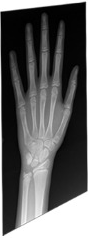
\includegraphics[scale=0.65]{misc/imgRadiografia.png}};
		%FLECHA
		\node[inner sep=0pt] (russell) at (0.55,1.95)
    {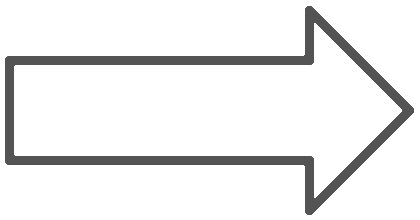
\includegraphics[scale=0.06]{misc/imgArrowOutline.png}};
		%PRIMER CUBO
		\draw[thick,-](1.5,1,1)--(1.5,3,1);
		\draw[thick,-](1.5,3,1)--(1.75,3,1);
		\draw[thick,-](1.75,3,1)--(1.75,1,1);
		\draw[thick,-](1.75,1,1)--(1.5,1,1);
		\draw[thick,-](1.5,3,1)--(1.5,3,-1);		
		\draw[thick,-](1.5,3,-1)--(1.75,3,-1);
		\draw[thick,-](1.75,3,-1)--(1.75,3,1);
		\draw[thick,-](1.75,3,-1)--(1.75,1,-1);
		\draw[thick,-](1.75,1,-1)--(1.75,1,1);
		%SEGUNDO RECTANGULO
		\draw[thick,-](4,1.5,1)--(4,2.5,1);
		\draw[thick,-](4,2.5,1)--(4,2.5,0);
		\draw[thick,-](4,2.5,0)--(4,1.5,0);
		\draw[thick,-](4,1.5,0)--(4,1.5,1);
		%UNIONES ENTRE 1° Y 2° FIGURA
		\draw[thick,dashed,-](1.75,3,1)--(4,2.5,1);
		\draw[thick,dashed,-](1.75,1,1)--(4,1.5,1);
		\draw[thick,dashed,-](1.75,3,-1)--(4,2.5,0);
		\draw[thick,dashed,-](1.75,1,-1)--(4,1.5,0);
		%FLECHA
		\draw[thick,->](4.6,2.3,1)--(5.75,2.3,1);
		%TERCER RECTANGULO 
		\draw[thick,-](6,1.25,1)--(6,3.25,1);
		\draw[thick,-](6,3.25,1)--(6.25,3.25,1);
		\draw[thick,-](6.25,3.25,1)--(6.25,1.25,1);
		\draw[thick,-](6.25,1.25,1)--(6,1.25,1);
		%FLECHA
		\draw[thick,->](6.35,2.3,1)--(7.9,2.3,1);
		%CUARTO RECTANGULO 
		\draw[thick,-](8,1.25,1)--(8,3.25,1);
		\draw[thick,-](8,3.25,1)--(8.25,3.25,1);
		\draw[thick,-](8.25,3.25,1)--(8.25,1.25,1);
		\draw[thick,-](8.25,1.25,1)--(8,1.25,1);
		%FLECHA
		\draw[thick,->](8.35,2.3,1)--(9.125,2.3,1);
		%QUINTO RECTANGULO 
		\draw[thick,-](9.225,1.25,1)--(9.225,3.25,1);
		\draw[thick,-](9.225,3.25,1)--(9.475,3.25,1);
		\draw[thick,-](9.475,3.25,1)--(9.475,1.25,1);
		\draw[thick,-](9.475,1.25,1)--(9.225,1.25,1);
		%FLECHA
		\draw[thick,->](9.575,2.3,1)--(10.25,2.3,1);
		%SEXTO RECTANGULO 
		\draw[thick,-](10.35,1.25,1)--(10.35,3.25,1);
		\draw[thick,-](10.35,3.25,1)--(10.60,3.25,1);
		\draw[thick,-](10.60,3.25,1)--(10.60,1.25,1);
		\draw[thick,-](10.60,1.25,1)--(10.35,1.25,1);
		%FLECHA
		\draw[thick,->](10.7,2.3,1)--(11.375,2.3,1);
		%SEPTIMO RECTANGULO 
		\draw[thick,-](11.475,1.25,1)--(11.475,3.25,1);
		\draw[thick,-](11.475,3.25,1)--(11.725,3.25,1);
		\draw[thick,-](11.725,3.25,1)--(11.725,1.25,1);
		\draw[thick,-](11.725,1.25,1)--(11.475,1.25,1);
		%FLECHA
		\draw[thick,->](11.825,2.3,1)--(12.5,2.3,1);
		%OCTAVO RECTANGULO 
		\draw[thick,-](12.6,1.5,1)--(12.6,3,1);
		\draw[thick,-](12.6,3,1)--(12.85,3,1);
		\draw[thick,-](12.85,3,1)--(12.85,1.5,1);
		\draw[thick,-](12.85,1.5,1)--(12.6,1.5,1);
		%FLECHA
		\draw[thick,->](12.95,2.3,1)--(13.625,2.3,1);
		%NOVENO RECTANGULO 
		\draw[thick,-](13.725,1.5,1)--(13.725,3,1);
		\draw[thick,-](13.725,3,1)--(13.975,3,1);
		\draw[thick,-](13.975,3,1)--(13.975,1.5,1);
		\draw[thick,-](13.975,1.5,1)--(13.725,1.5,1);
		%FLECHA
		%\draw[thick,->](14.075,2.3,1)--(14.9,2.3,1);
		%DECIMO RECTANGULO 
		%\draw[thick,-](15,1.7,1)--(15,2.8,1);
		%\draw[thick,-](15,2.8,1)--(15.25,2.8,1);
		%\draw[thick,-](15.25,2.8,1)--(15.25,1.7,1);
		%\draw[thick,-](15.25,1.7,1)--(15,1.7,1);
		%FLECHA HACERLA DOBLE
		\node[inner sep=0pt] (russell) at (13.975,1.88)
    {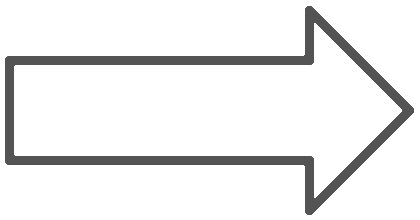
\includegraphics[scale=0.04]{misc/imgArrowOutline.png}};
		%ONCEAVO RECTANGULO 
		\draw[thick,-](15,1.9,1)--(15,2.6,1);
		\draw[thick,-](15,2.6,1)--(17,2.6,1);
		\draw[thick,-](17,2.6,1)--(17,1.9,1);
		\draw[thick,-](17,1.9,1)--(15,1.9,1);
		%TEXTOS
		\node[scale=0.65] at (15.65,1.98) {Y};
		\node[scale=0.65] at (15.65,1.7) {edad ósea estimada};
		\node[scale=1] at (5.75,0.68) {\ding{115}};
		\node[scale=0.75] at (5.7,0.35) {salida rn50 1000};
		\node[scale=1] at (7.75,0.68) {\ding{115}};
		\node[scale=0.75] at (7.8,0.35) {densa 1000 relu};
		\node[scale=1] at (8.95,3.1) {\ding{116}};
		\node[scale=0.75] at (8.95,3.4) {dropout 0.2};
		\node[scale=1] at (10.1,0.68) {\ding{115}};
		\node[scale=0.75] at (10.1,0.35) {densa 1000 relu};
		\node[scale=1] at (11.22,3.1) {\ding{116}};
		\node[scale=0.75] at (11.25,3.4) {dropout 0.2};
		\node[scale=1] at (12.35,0.9) {\ding{115}};
		\node[scale=0.75] at (12.4,0.6) {densa 240 relu};
		\node[scale=1] at (13.457,2.8) {\ding{116}};
		\node[scale=0.75] at (13.4,3.1) {densa 1 relu};
		%\node[scale=1] at (14.75,1.1) {\ding{115}};
		%\node[scale=0.75] at (14.9,0.8) {densa 1 regresión};
		\node[scale=1] at (4.2,3.2) {ResNet-50};
		\node[scale=1.4] at (3.5,4.5) {Convolución};
		\node[scale=1.4] at (10,4.5) {Capas totalmente conectadas};
		\node[inner sep=0pt] (russell) at (3.35,3.75)
    {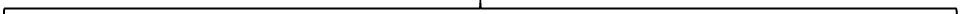
\includegraphics[width=4.5cm,height=0.25cm]{misc/imgLlave.png}};
		\node[inner sep=0pt] (russell) at (10,3.75)
    {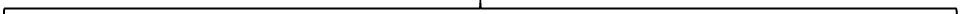
\includegraphics[width=9cm,height=0.25cm]{misc/imgLlave.png}};
	\end{tikzpicture}
\end{adjustbox}
\end{center}
 \caption{Sistema propuesto especializado en género}
  \end{subfigure}%
\\
\\
\\
\begin{subfigure}{.5\textwidth}
  \centering
\begin{center}
\begin{adjustbox}{width=\columnwidth}
	\begin{tikzpicture}[scale = 1]	
		\node[inner sep=0pt] (russell) at (-0.6,3.05)
    {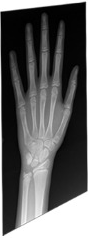
\includegraphics[scale=0.65]{misc/imgRadiografia.png}};
		%FLECHA
		\node[inner sep=0pt] (russell) at (0.55,3.2)
    {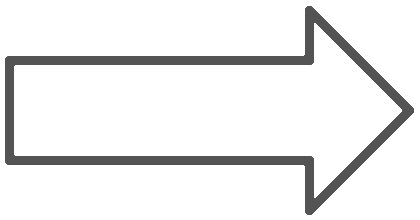
\includegraphics[scale=0.06]{misc/imgArrowOutline.png}};
		%PRIMER CUBO
		\draw[thick,-](1.5,2.25,1)--(1.5,4.25,1);
		\draw[thick,-](1.5,4.25,1)--(1.75,4.25,1);
		\draw[thick,-](1.75,4.25,1)--(1.75,2.25,1);
		\draw[thick,-](1.75,2.25,1)--(1.5,2.25,1);
		\draw[thick,-](1.5,4.25,1)--(1.5,4.25,-1);		
		\draw[thick,-](1.5,4.25,-1)--(1.75,4.25,-1);
		\draw[thick,-](1.75,4.25,-1)--(1.75,4.25,1);
		\draw[thick,-](1.75,4.25,-1)--(1.75,2.25,-1);
		\draw[thick,-](1.75,2.25,-1)--(1.75,2.25,1);
		%SEGUNDO RECTANGULO
		\draw[thick,-](4,2.75,1)--(4,3.75,1);
		\draw[thick,-](4,3.75,1)--(4,3.75,0);
		\draw[thick,-](4,3.75,0)--(4,2.75,0);
		\draw[thick,-](4,2.75,0)--(4,2.75,1);
		%UNIONES ENTRE 1° Y 2° FIGURA
		\draw[thick,dashed,-](1.75,4.25,1)--(4,3.75,1);
		\draw[thick,dashed,-](1.75,2.25,1)--(4,2.75,1);
		\draw[thick,dashed,-](1.75,4.25,-1)--(4,3.75,0);
		\draw[thick,dashed,-](1.75,2.25,-1)--(4,2.75,0);
		%FLECHA
		\draw[thick,->](4.6,3.55,1)--(5.75,3.55,1);
		%TERCER RECTANGULO 
		\draw[thick,-](6,2.5,1)--(6,4.5,1);
		\draw[thick,-](6,4.5,1)--(6.25,4.5,1);
		\draw[thick,-](6.25,4.5,1)--(6.25,2.5,1);
		\draw[thick,-](6.25,2.5,1)--(6,2.5,1);
		%FLECHA
		\draw[thick,->](6.35,3.55,1)--(7.6,2.3,1);
		%CUADRADO inferior
		\draw[thick,-](2.55,-0.75,1)--(2.55,1.25,1);
		\draw[thick,-](2.55,1.25,1)--(4.55,1.25,1);
		\draw[thick,-](4.55,1.25,1)--(4.55,-0.75,1);
		\draw[thick,-](4.55,-0.75,1)--(2.55,-0.75,1);
		%FLECHA inferior
		\node[inner sep=0pt] (russell) at (4.85,-0.1)
    {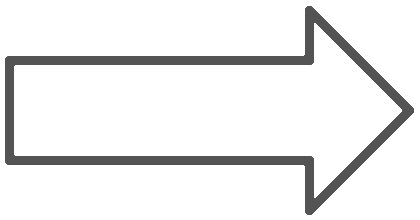
\includegraphics[scale=0.06]{misc/imgArrowOutline.png}};
		%RECTANGULO inferior
		\draw[thick,-](5.85,-0.25,1)--(5.85,0.75,1);
		\draw[thick,-](5.85,0.75,1)--(6.1,0.75,1);
		\draw[thick,-](6.1,0.755,1)--(6.1,-0.25,1);
		\draw[thick,-](6.1,-0.25,1)--(5.85,-0.25,1);
		%FLECHA diagonal desde inferior a superior
		\draw[thick,->](6.2,0.25,1)--(7.6,2.1,1);
		%CUARTO RECTANGULO 
		\draw[thick,-](7.7,1.25,1)--(7.7,3.25,1);
		\draw[thick,-](7.7,3.25,1)--(7.95,3.25,1);
		\draw[thick,-](7.95,3.25,1)--(7.95,1.25,1);
		\draw[thick,-](7.95,1.25,1)--(7.7,1.25,1);
		%FLECHA
		\draw[thick,->](8.05,2.3,1)--(8.65,2.3,1);
		%QUINTO RECTANGULO 
		\draw[thick,-](8.75,1.25,1)--(8.75,3.25,1);
		\draw[thick,-](8.75,3.25,1)--(9,3.25,1);
		\draw[thick,-](9,3.25,1)--(9,1.25,1);
		\draw[thick,-](9,1.25,1)--(8.75,1.25,1);
		%FLECHA
		\draw[thick,->](9.1,2.3,1)--(9.7,2.3,1);
		%SEXTO RECTANGULO 
		\draw[thick,-](9.8,1.25,1)--(9.8,3.25,1);
		\draw[thick,-](9.8,3.25,1)--(10.05,3.25,1);
		\draw[thick,-](10.05,3.25,1)--(10.05,1.25,1);
		\draw[thick,-](10.05,1.25,1)--(9.8,1.25,1);
		%FLECHA
		\draw[thick,->](10.15,2.3,1)--(10.75,2.3,1);
		%SEXTO RECTANGULO 
		\draw[thick,-](10.85,1.25,1)--(10.85,3.25,1);
		\draw[thick,-](10.85,3.25,1)--(11.1,3.25,1);
		\draw[thick,-](11.1,3.25,1)--(11.1,1.25,1);
		\draw[thick,-](11.1,1.25,1)--(10.85,1.25,1);
		%FLECHA
		\draw[thick,->](11.2,2.3,1)--(11.8,2.3,1);
		%SEPTIMO RECTANGULO 
		\draw[thick,-](11.9,1.25,1)--(11.9,3.25,1);
		\draw[thick,-](11.9,3.25,1)--(12.15,3.25,1);
		\draw[thick,-](12.15,3.25,1)--(12.15,1.25,1);
		\draw[thick,-](12.15,1.25,1)--(11.9,1.25,1);
		%FLECHA
		\draw[thick,->](12.25,2.3,1)--(12.85,2.3,1);
		%OCTAVO RECTANGULO 
		\draw[thick,-](12.95,1.5,1)--(12.95,3,1);
		\draw[thick,-](12.95,3,1)--(13.2,3,1);
		\draw[thick,-](13.2,3,1)--(13.2,1.5,1);
		\draw[thick,-](13.2,1.5,1)--(12.95,1.5,1);
		%FLECHA
		\draw[thick,->](13.30,2.3,1)--(13.85,2.3,1);
		%NOVENO RECTANGULO 
		\draw[thick,-](14,1.5,1)--(14,3,1);
		\draw[thick,-](14,3,1)--(14.25,3,1);
		\draw[thick,-](14.25,3,1)--(14.25,1.5,1);
		\draw[thick,-](14.25,1.5,1)--(14,1.5,1);
		%FLECHA
		%\draw[thick,->](14.35,2.3,1)--(14.9,2.3,1);
		%DECIMO RECTANGULO 
		%\draw[thick,-](15,1.7,1)--(15,2.8,1);
		%\draw[thick,-](15,2.8,1)--(15.25,2.8,1);
		%\draw[thick,-](15.25,2.8,1)--(15.25,1.7,1);
		%\draw[thick,-](15.25,1.7,1)--(15,1.7,1);
		%FLECHA HACERLA DOBLE
		\node[inner sep=0pt] (russell) at (14.27,1.88)
    {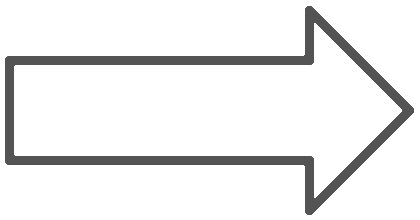
\includegraphics[scale=0.04]{misc/imgArrowOutline.png}};
		%ONCEAVO RECTANGULO 
		\draw[thick,-](15,1.9,1)--(15,2.6,1);
		\draw[thick,-](15,2.6,1)--(17,2.6,1);
		\draw[thick,-](17,2.6,1)--(17,1.9,1);
		\draw[thick,-](17,1.9,1)--(15,1.9,1);
		%TEXTOS
		\node[scale=0.65] at (15.6,1.98) {Y};
		\node[scale=0.65] at (15.6,1.7) {edad ósea estimada};
		\node[scale=1.4] at (3.2,0.25) {Género};
		\node[scale=1.4] at (3.2,-0.5) {M/F};
		\node[scale=1] at (5.6,-0.85) {\ding{115}};
		\node[scale=0.75] at (5.6,-1.15) {densa 32 relu};
		\node[scale=1] at (5.75,1.93) {\ding{115}};
		\node[scale=0.75] at (5.5,1.6) {salida rn50 1000};
		\node[scale=1] at (7.43,3.1) {\ding{116}};
		\node[scale=0.75] at (7.55,3.4) {concat 1032};
		\node[scale=1] at (8.5,0.68) {\ding{115}};
		\node[scale=0.75] at (8.5,0.35) {densa 1000 relu};
		\node[scale=1] at (9.53,3.1) {\ding{116}};
		\node[scale=0.75] at (9.53,3.4) {dropout 0.2};
		\node[scale=1] at (10.6,0.68) {\ding{115}};
		\node[scale=0.75] at (10.6,0.35) {densa 1000 relu};
		\node[scale=1] at (11.63,3.1) {\ding{116}};
		\node[scale=0.75] at (11.63,3.4) {dropout 0.2};
		\node[scale=1] at (12.7,0.9) {\ding{115}};
		\node[scale=0.75] at (12.7,0.6) {densa 240 relu};
		\node[scale=1] at (13.73,2.8) {\ding{116}};
		\node[scale=0.75] at (13.73,3.1) {densa 1 relu};
		%\node[scale=1] at (14.75,1.1) {\ding{115}};
		%\node[scale=0.75] at (14.9,0.8) {densa 1 regresión};
		\node[scale=1] at (4.2,4.45) {ResNet-50};
		\node[scale=1.4] at (3.5,5.75) {Convolución};
		\node[scale=1.4] at (10,5.75) {Capas totalmente conectadas};
		\node[inner sep=0pt] (russell) at (3.35,5)
    {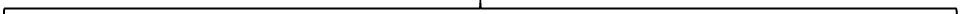
\includegraphics[width=4.5cm,height=0.25cm]{misc/imgLlave.png}};
		\node[inner sep=0pt] (russell) at (10,5)
    {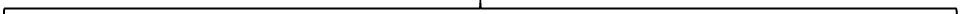
\includegraphics[width=8.5cm,height=0.25cm]{misc/imgLlave.png}};
	\end{tikzpicture}
\end{adjustbox}
\end{center}
 \caption{Sistema propuesto generalizado para ambos géneros}
  \end{subfigure}
   \caption{Sistemas propuestos}
   \label{fig:sistemas}
\end{figure}


\section{Resultados del experimento}
Para los experimentos realizados se ha calculado el MAE resultante en cada uno de los sistemas propuestos con un conjunto de datos de radiografías masculinas y/o femeninas según corresponda. Los resultados se muestran en el Cuadro~\ref{table:tablaResultados}. En cada fila se muestran los MAE en meses resultantes para cada sistema. La primer columna especifica el sistema utilizado. Segunda columna el MAE resultante para el conjunto de radiografías femeninas. Tercer columna el MAE resultante para el conjunto de radiografías masculinas.
Puede observarse que el sistema generalizado obtiene mejores resultados para ambos conjuntos de datos. El sistema generalizado presenta mayor precisión con respecto al sistema especializado en radiografías femeninas en \textasciitilde{}1.066 meses. También presenta mayor presición con respecto al sistema especializado en radiografías masculinas en \textasciitilde{}0.571 meses.
\begin{table}[]
\centering
\resizebox{.48\textwidth}{!}{%
\begin{tabular}{l|>{\centering\arraybackslash}p{1in}>{\centering\arraybackslash}m{1in}ll}
 							&Femeninas	&Masculinas \\ \hline
 Generalizado				&9.326	&9.120	\\ \hline
 Especializado Femeninas	&10.392	&-  		\\ \hline
 Especializado Masculinas	&-			&9.691 
\end{tabular}
}
\caption{MAE en meses de los sistemas de acuerdo al género de radiografía utilizado}
\label{table:tablaResultados}
\end{table}

\section{Conclusiones y Trabajo Futuro}

En esta sección se presentan conclusiones sobre la experimentación realizada y pasos a seguir para aumentar la precisión de los sistemas tratados.

\subsection{Conclusiones}
Nuestra motivación en esta experimentación fue evaluar los diferentes comportamientos que puede presentar una red neuronal de acuerdo a variaciones en el conjunto de datos de entrada como así también los parámetros utilizados en la misma. Se han presentado los resultados obtenidos sobre los sistemas propuestos. Se ha observado que un sistema que acepte ambos géneros ha obtenido mayor precisión. Sin embargo, la pequeña diferencia en precisión observada al compararlo con los sistemas especializados da lugar a pensar mejoras que podrían disminuir tal diferencia. Además, se han desarrollado arquitecturas para la extracción de patrones y estimación de edad de una radiografía de mano y muñeca pediátrica que podría ser de gran utilidad para aquellas personas interesadas en abordar problemáticas similares, como así también en el ámbito de la medicina a través de su implementación en instituciones de salud, como Hospitales o Sanatorios, para asistir en la labor de pediátras, endocrinólogos, radiólogos y/u otros especialistas. 


\subsection{Trabajo Futuro}
En una segunda fase de experimentación el desafío se centra en aumentar la precisión de los sistemas. El módulo de preprocesamiento actual ha probado su utilidad aumentando la precisión de los modelos en 0,2 meses. En una segunda fase se reemplazará el módulo por una red neuronal que realice las mismas funciones con mayor precisión, lo que se estima que disminuirá el error de los modelos. Además, se continuará experimentando variaciones estructurales en el etapa de capas totalmente conectadas, como así también variaciones en la etapa convolucional. En cuanto al conjunto de datos, se aplicarán técnicas de aumento de datos (data augmentation) para incrementar la cantidad de radiografías con las que sería posible entrenar los sistemas.


\begin{thebibliography}{00}
\bibitem{AproachToSkeletalMaturation} 
Zerin, J. M., \& Hernandez, R. J. (1991). 
\textit{Approach to skeletal maturation}. 
Hand clinics, 7(1), 53-62.

\bibitem{GP} 
Greulich, W. W., Pyle, S. I., \& Todd, T. W. (1959).
\textit{Radiographic atlas of skeletal development of the hand and wrist}. 
(Vol. 2, pp. 150-159). Stanford: Stanford university press.

\bibitem{TW3} 
Tanner, J. M., Healy, M. R. J., Goldstein, H., \& Cameron, N. (2001).
\textit{Assessment of skeletal maturity and prediction of adult height (TW3 method)}. 
WB Saunders, London, 243-254.

\bibitem{GP_variability} 
Berst, M. J., Dolan, L., Bogdanowicz, M. M., Stevens, M. A., Chow, S., \& Brandser, E. A. (2001).
\textit{Effect of knowledge of chronologic age on the variability of pediatric bone age determined using the Greulich and Pyle standards}. 
American Journal of Roentgenology, 176(2), 507-510.

\bibitem{DeepLearningInBiology} 
Ching, T., Himmelstein, D. S., Beaulieu-Jones, B. K., Kalinin, A. A., Do, B. T., Way, G. P., ... \& Xie, W. (2018).
\textit{Opportunities and obstacles for deep learning in biology and medicine}.
Journal of The Royal Society Interface, 15(141), 20170387.

\bibitem{DeepLearning} 
LeCun, Y., Bengio, Y., \& Hinton, G. (2015).
\textit{Deep learning}.
Nature, 521(7553), 436.

\bibitem{DeepLearningInDiabetics}
Rakhlin, A. (2018).
\textit{Diabetic Retinopathy detection through integration of Deep Learning classification framework}.
bioRxiv, 225508.

\bibitem{DeepLearningInHeartDiseases}
Korshunova, I. (2017).
\textit{Diagnosing heart diseases with deep neural networks}.
\\\texttt{\url{https://irakorshunova.github.io/2016/03/15/heart.html}}, accedido 29 de Julio de 2017.

\bibitem{DeepLearningLungCancer}
Daniel Hammack and Julian de Wit. (2017)
\textit{2017 Data Science Bowl, Predicting Lung Cancer: 2nd place solution write-up}.
\\\texttt{\url{http://blog.kaggle.com/2017/06/29/2017-data-science-bowl-predicting-lung-cancer-2nd-place-solution-write-up-daniel-hammack-and-julian-de-wit/}}, accedido 29 de Julio de 2017.

\bibitem{DeepLearningAssesingSkeletalMaturity1}
Larson, D. B., Chen, M. C., Lungren, M. P., Halabi, S. S., Stence, N. V., \& Langlotz, C. P. (2017).
\textit{Performance of a deep-learning neural network model in assessing skeletal maturity on pediatric hand radiographs}.
Radiology, 287(1), 313-322.

\bibitem{DeepLearningAssesingSkeletalMaturity2}
Lee, H., Tajmir, S., Lee, J., Zissen, M., Yeshiwas, B. A., Alkasab, T. K., ... \& Do, S. (2017).
\textit{Fully automated deep learning system for bone age assessment}.
Journal of digital imaging, 30(4), 427-441.

\bibitem{DeepLearningAssesingSkeletalMaturity3}
Spampinato, C., Palazzo, S., Giordano, D., Aldinucci, M., \& Leonardi, R. (2017).
\textit{Deep learning for automated skeletal bone age assessment in X-ray images}.
Medical image analysis, 36, 41-51.

\bibitem{RSNAChallenge}
\textit{RSNA Pediatric Bone Age Challenge}.
\\\texttt{\url{http://rsnachallenges.cloudapp.net/competitions/4}}, accedido 29 de julio de 2017.

\bibitem{RSNADataSet}
Stanford University Artificial Intelligence in Medicine \& Imaging (2017).
\textit{Bone age images used in the 2017 RSNA bone age challenge competition}.
\\\texttt{\url{https://aimi.stanford.edu/available-labeled-medical-datasets}}, accedido 29 de julio de 2017.

\bibitem{AtlasMedicina}
Gilroy, A.M., MacPherson B.R., Ross L.M., Schünke M., Schulte E., Schumacher U., Voll M., \& Wesker K. (2008).
\textit{Prometheus. Atlas de Anatomía}.
pp 298.

\bibitem{ResNet}
He, K., Zhang, X., Ren, S., \& Sun, J. (2016). 
\textit{Deep residual learning for image recognition}.
In Proceedings of the IEEE conference on computer vision and pattern recognition (pp. 770-778).

\bibitem{Imagenet}
Deng, J., Dong, W., Socher, R., Li, L. J., Li, K., \& Fei-Fei, L. (2009, June). 
\textit{Imagenet: A large-scale hierarchical image database}. In Computer Vision and Pattern Recognition, 2009. CVPR 2009. IEEE Conference on (pp. 248-255). Ieee.


\bibitem{InceptionV3}
Szegedy, C., Vanhoucke, V., Ioffe, S., Shlens, J., \& Wojna, Z. (2016). 
\textit{Rethinking the inception architecture for computer vision}. In Proceedings of the IEEE conference on computer vision and pattern recognition (pp. 2818-2826).


\bibitem{Xception}
Chollet, F. (2017).
\textit{Xception: Deep learning with depthwise separable convolutions}. arXiv preprint, 1610-02357.
\end{thebibliography}


\end{document}
